\subsection{UniProt}
\label{uniprotdb}

\subsubsection{Introduction}
It is important to restate the goal of the XMLPipeDB project before understanding 
the important role UniProt played in the project: To create a reusable tool set 
that given genomic sequencing data for an organism in XML and a schema for that 
XML document could output a working GenMAPP gene database for that organism.  During
the beginning phases of the project, there was only one project, XMLPipeDB, and it
made use of the schema provided by the UniProt Consortium~\cite{uniprotWeb}.  However,
it soon became evident that the project could be designed in a manner that would 
allow a wider audience the use of our tool.  The first phase was xsd2db, thoroughly
discussed in Section~\ref{xsd2db}.  xsd2db allowed for the use of any schema
to create the necessary JAXB objects and hibernate mappings.  However, we still
needed to create a tool for the Bioinformatics community.  At that point, uniprotdb
was born.  

\subsubsection{Design}
Before the project was split into a variety of subprojects, XMLPipeDB offered
the ability to use the UniProt schema and created the necessary JAXB objects
and hibernate mappings.  It created these files in default directories that 
are called out in the hyperjaxb2 template project~\cite{hyperjaxb}.  Once it was
determined that we wanted to allow for groups to use our tool outside the 
Bioinformatics community, uniprotdb became its own subproject.  uniprotdb
would be created from the output of xsd2db.  It would contain the UniProt schema,
SQL DDL file that corresponds to the schema, the JAXB objects, and the hibernate
mappings.  
The layout 
shown in Figure~\ref{fig:uniprotLayout} was what we hoped uniprotdb would look like.  

\begin{figure}[htp]
\centering
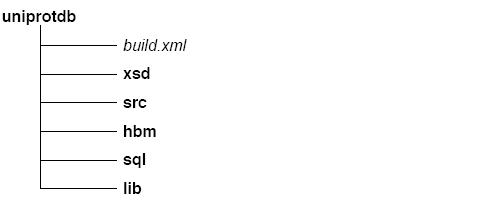
\includegraphics[scale=1.0]{Images/uniprotLayout.jpg}
\caption{\small \sl The uniprotdb layout.} 
\label{fig:uniprotLayout}
\end{figure}

The build file would have the following capabilities:
\begin{itemize}
  \item \textit{compile} compiles the JAXB objects located within the src directory with help from any necessary jars located in the lib directory

  \item \textit{jar} compile and create a jar file containing the class files derived from the src directory and the hibernate mappings located within the hbm directory
  
  \item \textit{clean} eliminates all the products of a previous build.  
\end{itemize}

The jar file created as a result of a build would later be used in the gmbuilder 
subproject, thoroughly outlined in Section~\ref{gmbuilder}.  Once uniprotdb was
created, we would have been one step closer to creating a GenMAPP usable, gene 
database.  

\subsubsection{Implementation}
%discuss phases of the post processor and the failed usage of hibernate bindings

\subsubsection{Improvements}

\subsubsection{Conclusion}
 
